%==============================================
% ORULATEX ASSIGNMENT TEMPLATE
%==============================================

%==============================================
% BEGINNING OF PREAMBLE
%==============================================
\documentclass[12pt,letterpaper]{orulawork}
%==============================================

%==============================================
% ASSIGNMENT AND TEACHER INFORMATION (Update this)
%==============================================
\teacher{Stu D. Baker}
\assignment{Take-Home Assignment}
\coursecode{Math 331}
\coursename{Systems of Equations}
\topics{Graphing, Systems of Quadratic Equations}
\duedate{N/A}
%==============================================

\newif\ifanswerkey
\newcommand{\answer}[1]{%
	\ifanswerkey%
	{\\\color{red}[Ans: #1]}%
	\fi%
}
%\answerkeytrue

%==============================================
% BEGINNING OF DOCUMENT
%==============================================
\begin{document}
%==============================================

\instructions{Complete all of the following exercises. These are extra practice questions and are not to be handed-in.}

\begin{question}
	Graph the equation $y=3-2x$ by plotting two points on the line plus a third as a check.
	\begin{center}
		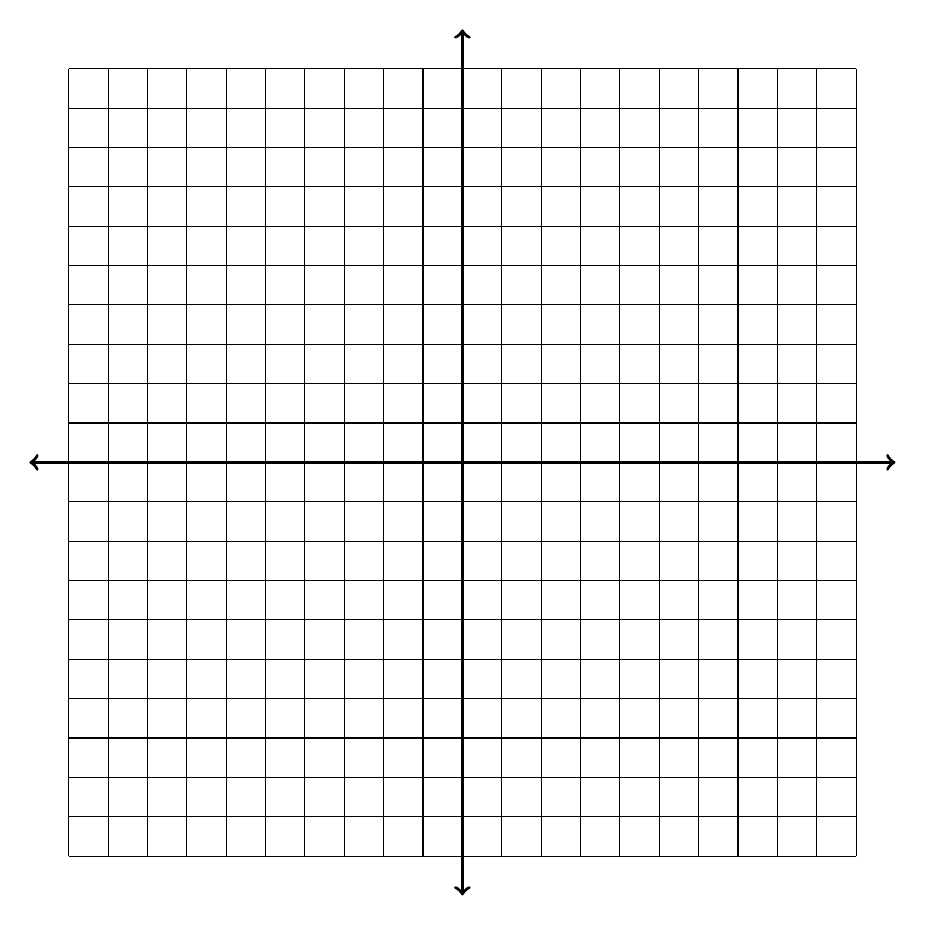
\begin{tikzpicture}
		\draw (-5.0,-5.0) -- (5.0,-5.0);
		\draw (-5.0,-4.5) -- (5.0,-4.5);
		\draw (-5.0,-4.0) -- (5.0,-4.0);
		\draw (-5.0,-3.5) -- (5.0,-3.5);
		\draw (-5.0,-3.0) -- (5.0,-3.0);
		\draw (-5.0,-2.5) -- (5.0,-2.5);
		\draw (-5.0,-2.0) -- (5.0,-2.0);
		\draw (-5.0,-1.5) -- (5.0,-1.5);
		\draw (-5.0,-1.0) -- (5.0,-1.0);
		\draw (-5.0,-0.5) -- (5.0,-0.5);
		\draw [<->,very thick] (-5.5,0.0) -- (5.5,0.0);
		\draw (-5.0,0.5) -- (5.0,0.5);
		\draw (-5.0,1.0) -- (5.0,1.0);
		\draw (-5.0,1.5) -- (5.0,1.5);
		\draw (-5.0,2.0) -- (5.0,2.0);
		\draw (-5.0,2.5) -- (5.0,2.5);
		\draw (-5.0,3.0) -- (5.0,3.0);
		\draw (-5.0,3.5) -- (5.0,3.5);
		\draw (-5.0,4.0) -- (5.0,4.0);
		\draw (-5.0,4.5) -- (5.0,4.5);
		\draw (-5.0,5.0) -- (5.0,5.0);
		\draw (-5.0,-5.0) -- (-5.0,5.0);
		\draw (-4.5,-5.0) -- (-4.5,5.0);
		\draw (-4.0,-5.0) -- (-4.0,5.0);
		\draw (-3.5,-5.0) -- (-3.5,5.0);
		\draw (-3.0,-5.0) -- (-3.0,5.0);
		\draw (-2.5,-5.0) -- (-2.5,5.0);
		\draw (-2.0,-5.0) -- (-2.0,5.0);
		\draw (-1.5,-5.0) -- (-1.5,5.0);
		\draw (-1.0,-5.0) -- (-1.0,5.0);
		\draw (-0.5,-5.0) -- (-0.5,5.0);
		\draw [<->,very thick] (0.0,-5.5) -- (0.0,5.5);
		\draw (0.5,-5.0) -- (0.5,5.0);
		\draw (1.0,-5.0) -- (1.0,5.0);
		\draw (1.5,-5.0) -- (1.5,5.0);
		\draw (2.0,-5.0) -- (2.0,5.0);
		\draw (2.5,-5.0) -- (2.5,5.0);
		\draw (3.0,-5.0) -- (3.0,5.0);
		\draw (3.5,-5.0) -- (3.5,5.0);
		\draw (4.0,-5.0) -- (4.0,5.0);
		\draw (4.5,-5.0) -- (4.5,5.0);
		\draw (5.0,-5.0) -- (5.0,5.0);
		\ifanswerkey
			\draw [red,fill=red] (0,1.5) circle (.125) ;
			\draw [red,fill=red] (0.75,0) circle (.125) ;
			\draw [thick,<->,red] (-1.5,4.5) -- (2.5,-3.5);
		\fi
		\end{tikzpicture}
	\end{center}
\end{question}

\begin{question}
	Find the slope of each straight line.
	\begin{exercises}
		\item Rise = $4$; run = $2$ \answer{$\text{Slope}=2$}
		\item Connecting $(3,-3)$ \\and $(-6,2)$ \answer{$\text{Slope}=-\frac{5}{9}$}
	\end{exercises}
\end{question}

\begin{question}
	Write the equation of the straight line with slope = $-1$ and $y$-intercept = $2$ in slope-intercept form and make a graph. \answer{$y=-x+2$}
	\begin{center}
		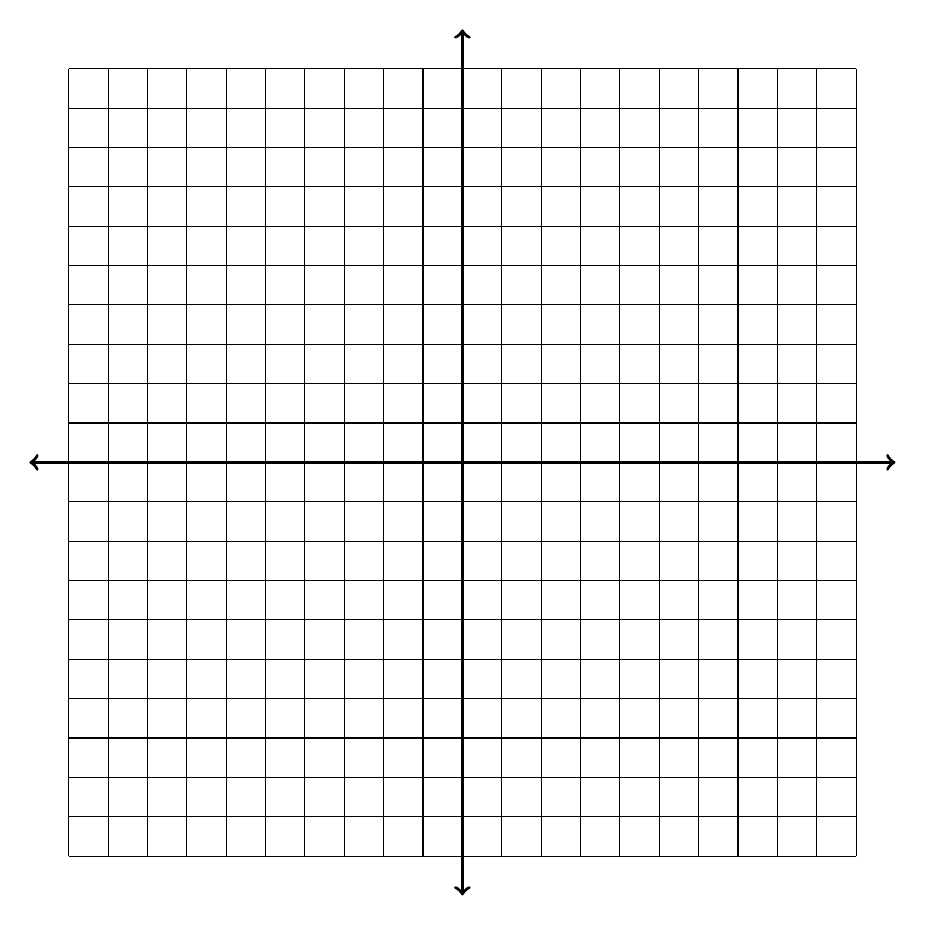
\begin{tikzpicture}
		\draw (-5.0,-5.0) -- (5.0,-5.0);
		\draw (-5.0,-4.5) -- (5.0,-4.5);
		\draw (-5.0,-4.0) -- (5.0,-4.0);
		\draw (-5.0,-3.5) -- (5.0,-3.5);
		\draw (-5.0,-3.0) -- (5.0,-3.0);
		\draw (-5.0,-2.5) -- (5.0,-2.5);
		\draw (-5.0,-2.0) -- (5.0,-2.0);
		\draw (-5.0,-1.5) -- (5.0,-1.5);
		\draw (-5.0,-1.0) -- (5.0,-1.0);
		\draw (-5.0,-0.5) -- (5.0,-0.5);
		\draw [<->,very thick] (-5.5,0.0) -- (5.5,0.0);
		\draw (-5.0,0.5) -- (5.0,0.5);
		\draw (-5.0,1.0) -- (5.0,1.0);
		\draw (-5.0,1.5) -- (5.0,1.5);
		\draw (-5.0,2.0) -- (5.0,2.0);
		\draw (-5.0,2.5) -- (5.0,2.5);
		\draw (-5.0,3.0) -- (5.0,3.0);
		\draw (-5.0,3.5) -- (5.0,3.5);
		\draw (-5.0,4.0) -- (5.0,4.0);
		\draw (-5.0,4.5) -- (5.0,4.5);
		\draw (-5.0,5.0) -- (5.0,5.0);
		\draw (-5.0,-5.0) -- (-5.0,5.0);
		\draw (-4.5,-5.0) -- (-4.5,5.0);
		\draw (-4.0,-5.0) -- (-4.0,5.0);
		\draw (-3.5,-5.0) -- (-3.5,5.0);
		\draw (-3.0,-5.0) -- (-3.0,5.0);
		\draw (-2.5,-5.0) -- (-2.5,5.0);
		\draw (-2.0,-5.0) -- (-2.0,5.0);
		\draw (-1.5,-5.0) -- (-1.5,5.0);
		\draw (-1.0,-5.0) -- (-1.0,5.0);
		\draw (-0.5,-5.0) -- (-0.5,5.0);
		\draw [<->,very thick] (0.0,-5.5) -- (0.0,5.5);
		\draw (0.5,-5.0) -- (0.5,5.0);
		\draw (1.0,-5.0) -- (1.0,5.0);
		\draw (1.5,-5.0) -- (1.5,5.0);
		\draw (2.0,-5.0) -- (2.0,5.0);
		\draw (2.5,-5.0) -- (2.5,5.0);
		\draw (3.0,-5.0) -- (3.0,5.0);
		\draw (3.5,-5.0) -- (3.5,5.0);
		\draw (4.0,-5.0) -- (4.0,5.0);
		\draw (4.5,-5.0) -- (4.5,5.0);
		\draw (5.0,-5.0) -- (5.0,5.0);
		\ifanswerkey
			\draw [red,fill=red] (0,1) circle (.125) ;
			\draw [red,fill=red] (1,0) circle (.125) ;
			\draw [thick,<->,red] (-3.5,4.5) -- (3.5,-2.5);
		\fi
		\end{tikzpicture}
	\end{center}
\end{question}

\begin{question}
	Solve for $x$ and $y$.
	\begin{exercises}
		\item%
		\begin{eqnarray*}
			x-y & = & 4 \\
			x^2-y^2 & = & 32 \\
		\end{eqnarray*} \answer{$(6,2)$}
		\item%
		\begin{eqnarray*}
			2x^2+3y & = & 10 \\
			x^2-y & = & 8 \\
		\end{eqnarray*} \answer{$(2.61,-1.20)$ and $(-2.61,-1.20)$}
		\item%
		\begin{eqnarray*}
			x-y & = & 11 \\
			xy+28 & = & 0 \\
		\end{eqnarray*} \answer{$(4,-7)$ and $(7,-4)$}
	\end{exercises}
\end{question}

%==============================================
% END OF DOCUMENT
%==============================================
\end{document}
%==============================================